\documentclass[nobib]{tufte-handout}

%\\geometry{showframe}% for debugging purposes -- displays the margins

\newcommand{\bra}[1]{\left(#1\right)}
\usepackage{clrscode3e}
\usepackage{hyperref}
\usepackage[activate={true,nocompatibility},final,tracking=true,kerning=true,spacing=true,factor=1100,stretch=10,shrink=10]{microtype}
\usepackage{color}
\usepackage{xcolor}
\usepackage{listings}

% Define a custom command for definitions
\newcommand{\defn}[2]{\noindent\textbf{#1}:\ #2}

% Fixes captions and images being cut off
\usepackage{marginfix}

\usepackage{caption}
\DeclareCaptionFont{white}{\color{white}}
\DeclareCaptionFormat{listing}{\colorbox{gray}{\parbox{\textwidth}{#1#2#3}}}
\captionsetup[lstlisting]{format=listing,labelfont=white,textfont=white}

\usepackage{tikz}
\usepackage{amsmath,amsthm}
\usetikzlibrary{shapes}
\usetikzlibrary{positioning}
% Set up the images/graphics package
\usepackage{graphicx}
\setkeys{Gin}{width=\linewidth,totalheight=\textheight,keepaspectratio}
\graphicspath{{.}}

\title{Notes for ECE 26400 - Advanced C Programming}
\author[Ezekiel Ulrich]{Ezekiel Ulrich}
\date{\today}  % if the \date{} command is left out, the current date will be used

% The following package makes prettier tables.  We're all about the bling!
\usepackage{booktabs}

% The units package provides nice, non-stacked fractions and better spacing
% for units.
\usepackage{units}

% The fancyvrb package lets us customize the formatting of verbatim
% environments.  We use a slightly smaller font.
\usepackage{fancyvrb}
\fvset{fontsize=\normalsize}

% Small sections of multiple columns
\usepackage{multicol}

% These commands are used to pretty-print LaTeX commands
\newcommand{\doccmd}[1]{\texttt{\textbackslash#1}}% command name -- adds backslash automatically
\newcommand{\docopt}[1]{\ensuremath{\langle}\textrm{\textit{#1}}\ensuremath{\rangle}}% optional command argument
\newcommand{\docarg}[1]{\textrm{\textit{#1}}}% (required) command argument
\newenvironment{docspec}{\begin{quote}\noindent}{\end{quote}}% command specification environment
\newcommand{\docenv}[1]{\textsf{#1}}% environment name
\newcommand{\docpkg}[1]{\texttt{#1}}% package name
\newcommand{\doccls}[1]{\texttt{#1}}% document class name
\newcommand{\docclsopt}[1]{\texttt{#1}}% document class option name

\begin{document}

\maketitle

\begin{abstract}
These are lecture notes for fall 2023 ECE 26400 at Purdue. Modify, use, and distribute as you please.
\end{abstract}

\tableofcontents


\section{Course Introduction}
Continuation of a first programming course. 
Topics include files, structures, pointers, and the proper use of dynamic data structures
This class will be taught by Prof. Joy Xiaoqian Wang. There will be four online exams, 
weekly online quizzes, and 20 homework assignments. For more information, 
consult the syllabus \href{https://github.com/ezekielulrich/Notes/blob/d83855d25b40c224ce70b0b46ae6a86adc5a783f/ECE%20264%20Fall%202023%20Syllabus.pdf}{here}.

\pagebreak

\section{Tools}

\defn{UNIX System}{The environment we'll use in this course.}
No matter your machine, you can use the UNIX environment. 
Some common commands in UNIX-like systems are:
\marginnote{For a comprehensive list of UNIX commands, 
see \href{https://en.wikipedia.org/wiki/List_of_Unix_commands}{Wikipedia's excellent page}}
\begin{itemize}
   \item \texttt{ls} - List directory contents
   \item \texttt{cd} - Change directory
   \item \texttt{mkdir} - Make directory
   \item \texttt{rm} - Remove files or directories. Use -rf to recursively delete files regardless of permission
   \item \texttt{mv} - Move files or directories
   \item \texttt{diff} - Comparing two files and showing their difference. Use -w to ignore whitespace
   \item \texttt{cat} - Shows contents of file without opening
   \item \texttt{cp} - Create a copy of a file
   \item \texttt{[CTRL + U]} - Undoes what was last typed
   \item \texttt{chmod} - Change file permissions
   \item \texttt{chown} - Change file ownership
   \item \texttt{kill} - Terminate processes
   \item \texttt{ssh} - Secure shell remote login
   \item \texttt{scp} - Securely copy files between hosts
   \item \texttt{wget} - Download files from the web
   \item \texttt{find} - Search for files and directories
   \item \texttt{vim} - Powerful text editor
\end{itemize}

\noindent To use these, simply type them in bash. For example, ls
will print the contents of your directory. 

\begin{lstlisting}[language=bash,caption=Using ls]
   $ ls
   code-folder/   helloworld.c   homework/
\end{lstlisting}

\defn{Git for Version Control}{Distributed version control system.} Git 
helps you manage, store, and collaborate on your project. The 
"version control" refers to how Git stores previous versions
of your code, so unwanted changes can be reverted. Git is useful
for when several people work on a project at a time or when you want
to keep track of changes.  

%insert flowchart here

When using Git, you will have a staging area on your computer where
you directly edit your code, a local repository (or repo)
that tracks all the files associated with a project, and a remote repo
to store the project. For this class, the remote repo is what's
that's graded (sending TAs to check student computers took too long).

You code on your local repo 
and then push it to the remote repo. You can also pull updates 
from the remote repo to your local.
\begin{figure}
   \centering
   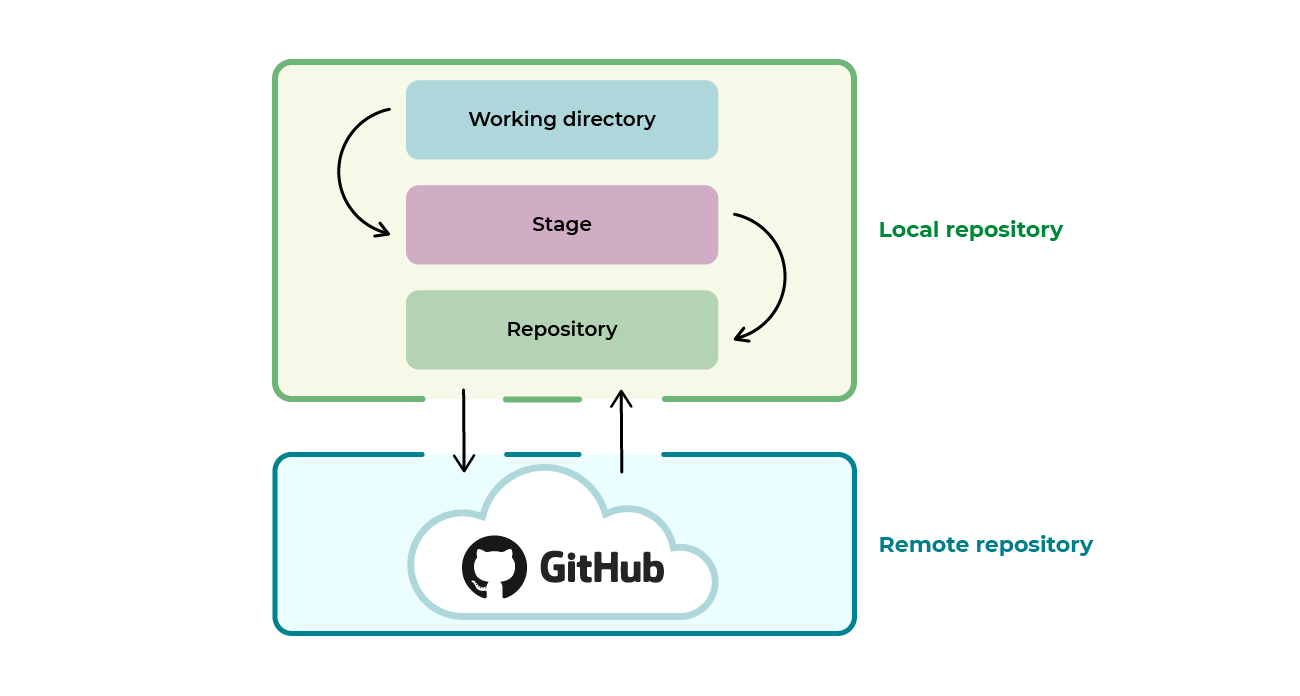
\includegraphics{images/workingdir-stage-local-remote.png}
   \caption{Layout of staging area, local repo, and remote repo}
   \label{fig:wdstagelocalremote} 
\end{figure}

Some common Git commands are:
\begin{itemize}
   \item \texttt{git push} - Replace what's on the remote repo with your local repo
   \item \texttt{git pull} - Replace your local repo with the remote repo
   \item \texttt{git init} - Creates a new Git repository
   \item \texttt{git clone} - Gets repo from specified url and copies to your machine, creating a new local repo
   \item \texttt{git add} - Adds file to staging area
   \item \texttt{git status} - Check what files in the working directory
   are added or committed
   \item \texttt{git log} - Check different versions of each project
   \item \texttt{git commit -m} - Moves changes from staging area to local repo. Use -m to add a message, and push
   to remote repo with \texttt{git push}
   \item \texttt{git reset} - Resets local repo to earlier version
\end{itemize}

\defn{GCC}{Compiles C code to executable program.}
Compiling a file with gcc is simple:
\begin{lstlisting}[language=bash,caption=Using gcc]
   $ gcc homework-one.c
\end{lstlisting}
Here are some useful gcc options:
\begin{itemize}
   \item \texttt{gcc [filename] -o [output name]} - Change executable file name
   \item \texttt{gcc -c [filename]} - Outputs as object file
   \item \texttt{gcc -o [filename]} - Outputs as executable file
   \item \texttt{gcc -g [filename]} - Generates debug information to be used by GDB debugger.
   \item \texttt{gcc -Wall} - Enables all compiler's warning messages. This option should always be used, in order to generate better code.
\end{itemize}

%how to link files together
% Conditional compilation
%-DSolution1 will tell the compiler to activate a
%#ifdef Solution1
%...
%#endif
%block

%also, #ifndef Solution1 ... #endif will activate if not that


\defn{Makefile}{Allows us to specify which options should be
used when gcc is called.}
\begin{lstlisting}[caption=Makefile]
   GCC=gccc
   CFLAGS=-std=c99 -g -Wall -Wshadow --pedantic -Wvla -Werror
   EXEC = sort
   TESTFLAGS = -DASCENDING

   all: main.c sort.c
         $(GCC) $(CFLAGS) -o $(EXEC) main.c sort.c

   # In general
   target: [dependencies]
         $(GCC) $(CFLAGS) -o $(EXEC) main.c sort.c

   clean:
         rm -f $(EXEC)
         rm -f *.o
\end{lstlisting}
The Makefile is invoked with the command "make" 
combined with a target in the terminal, like so
\begin{lstlisting}[caption=make clean]
   $ make clean
\end{lstlisting}

\defn{Header file}{Encapsulates formulas, function, and 
useful code for use in other programs. Uses ".h" extension.} For
compiler-included header files, include them in a preprocessor
directive with triangle brackets. For user-made header files,
use quotes instead. 
\begin{lstlisting}[caption=Header file usage]
   #include <stdio.h>
   #include "myheader.h"
\end{lstlisting}

\defn{GDB}{GNU Debugger, debugger that runs on many 
Unix-like systems and allows you to "see" what the computer
is doing as it compiles your code.}
Here are some useful gdb options:
\begin{itemize}
   \item \texttt{gdb prog} - Start gdb for debug
   \item \texttt{gdb -b filename.c : [line no. or function name]} - Adds a breakline location specifed by line no./function name
   \item \texttt{gdb -r [filename]} - 
   \item \texttt{gdb -n [filename]} - 
   \item \texttt{gdb -s [filename]} - 
\end{itemize}
The command to run the example file generated by -g is ./[name of example file].
The dot (.) signifies that the file is to be found in the current directory,
and the slash (/) refers to a specific file.

\end{document}
